
\documentclass[
	article,
	12pt,				
	oneside,
	a4paper,
	english,
	brazil
]{abntex2}


% Configuracoes de fonte
\usepackage{helvet}	
\renewcommand{\familydefault}{\sfdefault}		
\usepackage[utf8]{inputenc}
\usepackage[T1]{fontenc}		

\renewcommand{\ABNTEXchapterfontsize}{\LARGE} % Tamanho dos títulos dos capítulos

% Pacotes fundamentais 
\usepackage{indentfirst}		
\usepackage{color}				
\usepackage{graphicx}			
\usepackage{microtype}
\usepackage{listings}
\usepackage{pucmg}	% Customizacoes para os padroes PUC-MG
% ---

% Pacotes de citações
\usepackage[alf,abnt-emphasize=bf]{abntex2cite}	% Citações padrão ABNT

% Definições de estilo para a listagem de código
\lstloadlanguages{Python}

\definecolor{codegreen}{rgb}{0,0.6,0}
\definecolor{codegray}{rgb}{0.5,0.5,0.5}
\definecolor{codepurple}{rgb}{0.58,0,0.82}
\definecolor{backcolour}{rgb}{0.95,0.95,0.92}

\lstdefinestyle{estiloCodigo}{
    language=Python,
    backgroundcolor=\color{backcolour},   
    commentstyle=\color{codegreen},
    keywordstyle=\color{magenta},
    numberstyle=\tiny\color{codegray},
    stringstyle=\color{codepurple},
    basicstyle=\ttfamily,
    identifierstyle=\color{blue},
    breakatwhitespace=false,         
    breaklines=true,                 
    keepspaces=true,                 
    numbers=none,       
    numbersep=5pt,                  
    showspaces=false,                
    showstringspaces=false,
    showtabs=false,                  
    tabsize=2,
}

\lstset{style=estiloCodigo}
% ---

% Informações de dados para CAPA e FOLHA DE ROSTO
\titulo{\Large{CLASSIFICAÇÃO DE SEGMENTOS EM ATOS NORMATIVOS ATRAVÉS DE PROCESSAMENTO DE LINGUAGEM NATURAL}}
\autor{Leandro Coelho Correia}
\local{Salvador}
\data{2021}
\instituicao{Pontifícia Universidade Católica de Minas Gerais}
\departamento{Núcleo de Educação à Distância}
\filiacao{Pós-graduação em Inteligência Artificial e Aprendizado de Máquina}
\tipotrabalho{Relatório técnico}
\preambulo{Trabalho de Conclusão de Curso apresentado ao Curso de Especialização em Inteligência Artificial e Aprendizado de Máquina como requisito parcial à obtenção do título de especialista.}
% ---

% informações do PDF
\makeatletter
\hypersetup{
		pdftitle={\@title}, 
		pdfauthor={\@author},
    	pdfsubject={\imprimirpreambulo},
	    pdfcreator={LaTeX with abnTeX2},
		pdfkeywords={abnt}{latex}{abntex}{abntex2}{relatório técnico}, 
		bookmarksdepth=4
}
\makeatother
% --- 

% Espaçamentos
\setlength\afterchapskip{12pt} % Após o título dos capítulos
\setlength\beforesecskip{12pt} % Antes do título das seções
\setlength\aftersecskip{12pt} 	% Após o título das seções
\setlength{\parindent}{1.3cm} 	% Identação da primeira linha do parágrafo
\setlength{\parskip}{0.2cm}  	% Espaçamento entre um parágrafo e outro

% Compila o índice
\makeindex


% Início do documento
\begin{document}

\selectlanguage{brazil}

% Retira espaço extra obsoleto entre as frases.
\frenchspacing 

% ----------------------------------------------------------
% ELEMENTOS PRÉ-TEXTUAIS
% ----------------------------------------------------------
\pretextual

\imprimircapa
\imprimirfolhaderosto*

% inserir lista de ilustrações
\pdfbookmark[0]{\listfigurename}{lof}
\listoffigures*
\cleardoublepage
% ---

% inserir lista de tabelas
\pdfbookmark[0]{\listtablename}{lot}
\listoftables*
\cleardoublepage
% ---

% ---
% inserir o sumario
% ---
\pdfbookmark[0]{\contentsname}{toc}
\tableofcontents*
\cleardoublepage
% ---

% ------------------
% ELEMENTOS TEXTUAIS
% ------------------
\textual

\begingroup
\let\clearpage\relax
\section{Introdução}

\subsection{Atos Normativos}

A publicação de atos normativos é uma etapa fundamental do processo de gestão pública, pois formaliza e divulga para a sociedade as decisões do Governo Federal. A Receita Federal do Brasil (RFB) disponibiliza atos normativos através do sistema Normas \cite{Normas2021}, acessível publicamente através da Internet. Os atos são inicialmente publicados no Diário Oficial da União (DOU) através da Imprensa Nacional \cite{ImprensaNacional2021} e incluídos manualmente no sistema Normas.

Um ato normativo é composto por segmentos, trechos que possuem um significado próprio definido pelo Decreto N\textsuperscript{o} 10.139 de 28 de novembro de 2019 \cite{Decreto10139} e formatação específica definida pelo Manual de Redação da Presidência de República \cite{ManualRedacao2018}. A figura \ref{fig:segmentos} apresenta um ato normativo destacando alguns segmentos de tipos diferentes: a ementa destacada em vermelho, um segmento não identificado destacado em azul, alguns artigos em verde e o fecho em marrom ao final do ato. 

\begin{figure}[h]
	\caption{Exemplo de ato normativo com segmentos em destaque}
	\center
	\label{fig:segmentos}
	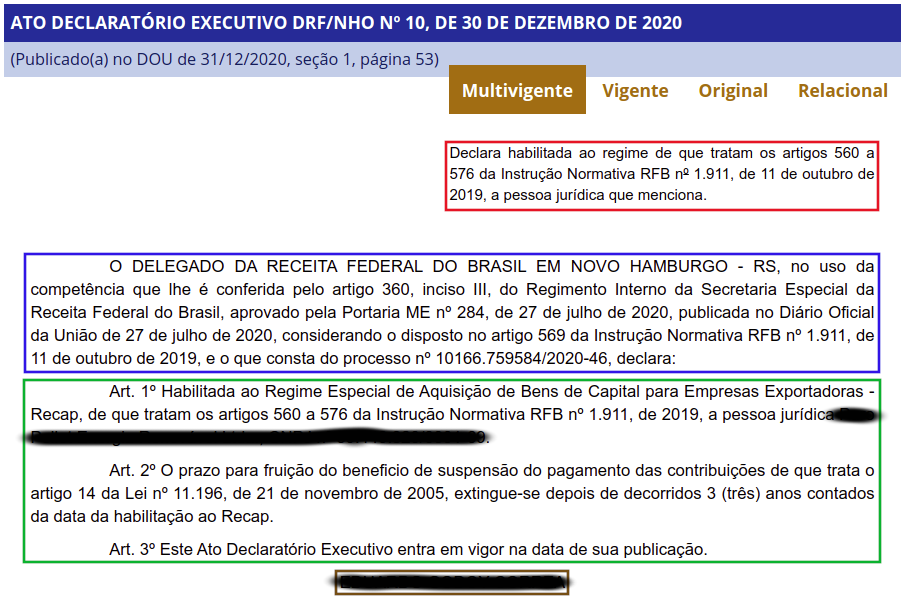
\includegraphics[scale=1.9]{introducao/segmentos.png}
	\fol{Normas2021}
\end{figure}

A classificação dos segmentos é uma etapa fundamental para o processo de inclusão de atos no sistema Normas, mas atualmente é realizada de forma totalmente manual, através de um procedimento que exige atenção e dedicação diária de uma equipe especializada da RFB. No período entre 2013 e 2020 foram incluídos aproximadamente 65 mil atos normativos compostos por mais de 600 mil segmentos, evidenciando um trabalho grande de classificação.

\subsection{Processamento de Linguagem Natural}

O Processamento de Linguagem Natural (PLN) é uma área da Ciência da Computação, fortemente relacionada com outras áreas de conhecimento como a Inteligência Artificial e o Aprendizado de Máquina, que pesquisa métodos para analisar, modelar e compreender a linguagem humana \cite{PracticalNLP2020}. Uma das tarefas de PLN é a classificação de textos que consiste em atribuir uma classe previamente conhecida a um texto informado. Alguns exemplos de classificação de textos são a identificação de \textit{spam} em mensagens eletrônicas e a análise de sentimentos em comentários de redes sociais. Para o escopo desta pesquisa os textos são os segmentos dos atos normativos e as classes são os diferentes tipos de segmento a exemplo da ementa, dos artigos, do fecho e do segmento não identificado mencionados anteriormente. 

\subsection{O Problema Proposto}

Este trabalho propôs a criação de um modelo de aprendizado de máquina, baseado em PLN, capaz de classificar automaticamente os segmentos de atos normativos provenientes do DOU, reduzindo o esforço e o tempo de inclusão dos atos no sistema Normas. A classificação automática de segmentos, além de contribuir para a otimização do trabalho da RFB, possibilita que os atos normativos sejam disponibilizados à sociedade em um intervalo de tempo menor.

Não fazem parte do escopo desta pesquisa a classificação do ato como um todo (pois o tipo do ato pode ser deduzido a partir do seu título através de heurísticas simples) nem o estudo dos relacionamentos entre os atos (uma funcionalidade complexa do sistema Normas que demanda uma pesquisa dedicada).

Para o desenvolvimento da pesquisa foi utilizada a linguagem de programação Python. A maior parte do código foi organizado em arquivos *.py contendo a lógica para realização das diversas etapas do fluxo de aprendizado de máquina. Além disso, foram criados dois Jupyter Notebooks responsáveis respectivamente pela realização da análise exploratória de dados e  orquestração das etapas do fluxo de aprendizado de máquina. Todo o código-fonte está disponível no repositório da pesquisa no Github\footnote{Segmentador Automático de Atos Normativos. Disponível em: \url{https://github.com/correialc/saan}. As versões das bibliotecas de software utilizadas estão descritas no arquivo \textit{requirements.txt} presente no repositório.}.





\section{Coleta de Dados}

Para a realização deste trabalho foi utilizado um conjunto de dados contendo 260.488 segmentos pertencentes a 20.821 atos do sistema Normas\footnote{Nem todos os atos do sistema Normas são de domínio público, mas todos os atos utilizados nesta pesquisa são públicos e podem ser acessados através da Internet, tanto pela Imprensa Nacional quanto pelo sistema Normas.}, relativos ao período de 01/01/2018 a 31/12/2020. Os dados estão em formato *.csv (arquivo extracacao-segmentos-atos.csv) e seguem a estrutura descrita na tabela \ref{tab:estrutura-conjunto-dados}.

\begin{table}[h!] 
\caption{Estrutura do conjunto de dados}
\label{tab:estrutura-conjunto-dados}
	\begin{center} 
		\begin{tabular}{|l|l|l|} 
			\hline ATRIBUTO & DESCRIÇÃO & TIPO \\
			\hline
			\hline id\textunderscore ato & Identificador do ato & Quantitativo Discreto \\ 
			\hline data\textunderscore  pub & Data de publicação do ato & Categórico Nominal \\ 
			\hline tipo\textunderscore  ato & Tipo do ato & Categórico Nominal \\
			\hline id\textunderscore seg & Identificador do segmento & Quantitativo Discreto \\
			\hline tipo\textunderscore seg & Tipo do segmento & Categórico Nominal \\
			\hline txt\textunderscore seg & Texto do segmento & Categórico Nominal \\
			\hline
		\end{tabular}
	\end{center}
	\fdp
\end{table}

Os atributos id\textunderscore ato, data\textunderscore  pub, tipo\textunderscore  ato e id\textunderscore seg foram utilizados somente para a análise exploratória e posterior limpeza dos dados. Os atributos relevantes para a criação do modelo de classificação foram txt\textunderscore seg (que representa o texto do segmento a ser classificado) e tipo\textunderscore seg (a classe ou \textit{label} do segmento).

A classe CargaDados (carga\textunderscore dados.py) é responsável por realizar a o processo de carga a partir do conjunto de dados de origem (extracacao-segmentos-atos.csv). A importação de dados foi realizada através do comando \textit{read\textunderscore csv} do Pandas. Os dados importados foram armazenados em uma instância da classe \textbf{Dados} definida no módulo \textbf{dados.py}. Essa classe foi utilizada ao longo de várias etapas do fluxo de aprendizado de máquina para armazenar dados temporários, atuando como um repositório de dados compartilhado.

O código a seguir apresenta um exemplo de execução da etapa de carga a partir notebook fluxo-ml.ipynb: 

\begin{lstlisting}
	dados = Dados()
	cg = CargaDados()
	cg.executar(dados)
	12:34:32 - Carregando dados de segmentos...
	12:34:32 - 206488 registros carregados.
\end{lstlisting}

Como a etapa de carga é a primeira a ser executada, é preciso inicialmente instanciar um objeto da classe Dados (esse objeto será utilizado ao longo de outras etapas além da carga). A seguir é criada uma instância da classe CargaDados, chamando o método ``executar'' passando o objeto de dados como parâmetro.



\section{Análise Exploratória}

A Análise Exploratória de Dados (AED) é uma etapa do fluxo de aprendizado de máquina que permite realizar uma exploração dos dados baseada em técnicas da Estatística Descritiva. Para essa etapa da pesquisa foi utilizado o notebook \textbf{analise-exploratoria.ipynb}. Por se tratar de uma atividade interativa, a utilização de um Jupyter Notebook se mostrou mais eficiente do que a utilização direta de um script Python.

\subsection{Valores Ausentes ou Inválidos}

A primeira investigação realizada foi a busca de valores valores ausentes. Foram encontrados 1.900 segmentos com valores ausentes para o atributo txt\textunderscore seg. Nos demais atributos não havia valores ausentes. A tabela \ref{tab:valores-ausentes} apresenta a quantidade de segmentos com valores ausentes por tipo de segmento.

\begin{table}[h] 
\caption{Valores ausentes por tipo de segmento}
\label{tab:valores-ausentes}
	\begin{center} 
		\begin{tabular}{lr} 
			\toprule			
			Tipo de Segmento & Valores Ausentes \\
			\midrule
			Anexo & 1.778 \\
			Não Identificado & 95 \\			
			Fecho & 21 \\
			Ementa & 2 \\			
			Artigo & 2 \\
			Título & 1 \\
			Alínea & 1 \\			
			\bottomrule
		\end{tabular}
	\end{center}
	\fdp
\end{table} 

Os segmentos do tipo Anexo representam 93,57\% dos segmentos com valores ausentes. Como esse tipo de segmento representa arquivos binários associados aos atos, todos os segmentos desse tipo podem ser descartados. Além dos 1.778 apresentados na tabela \ref{tab:valores-ausentes}, existem outros 5.771 segmentos do tipo anexo com texto desprezível (ponto, vírgula, nome de arquivo) totalizando 7.549 segmentos selecionados para exclusão durante a etapa de limpeza de dados. Os demais segmentos com valores ausentes representam 0,06\% do total (122/198.939) e foram também selecionados para exclusão.

Além dos valores ausentes, em diversos tipos de segmento foram identificados caracteres inválidos que precisaram ser removidos no processo de limpeza de dados, especialmente os caracteres de \textit{escape} e \textit{tags} HTML (exemplos: <br/>, \&ccedil, \&atilde).

\subsection{Distribuição de Atos e Segmentos \label{sec:dist-atos-segmentos}}

Um aspecto que chamou a atenção na exploração dos dados foi a predominância de Atos Declaratórios Executivos (ADE), representando 71,79\% (14.948 dos 20.821 atos analisados), seguido pelas Soluções de Consulta (SC) com 14,98\% e Portarias (PORT) com 10,60\%. Os demais tipos de ato representam juntos 2.63\% do total. A figura \ref{fig:atos-por-tipo-ato} evidencia essa distribuição.

\begin{figure}[h]
	\caption{Quantidade de atos por tipo de ato}
	\center
	\label{fig:atos-por-tipo-ato}
	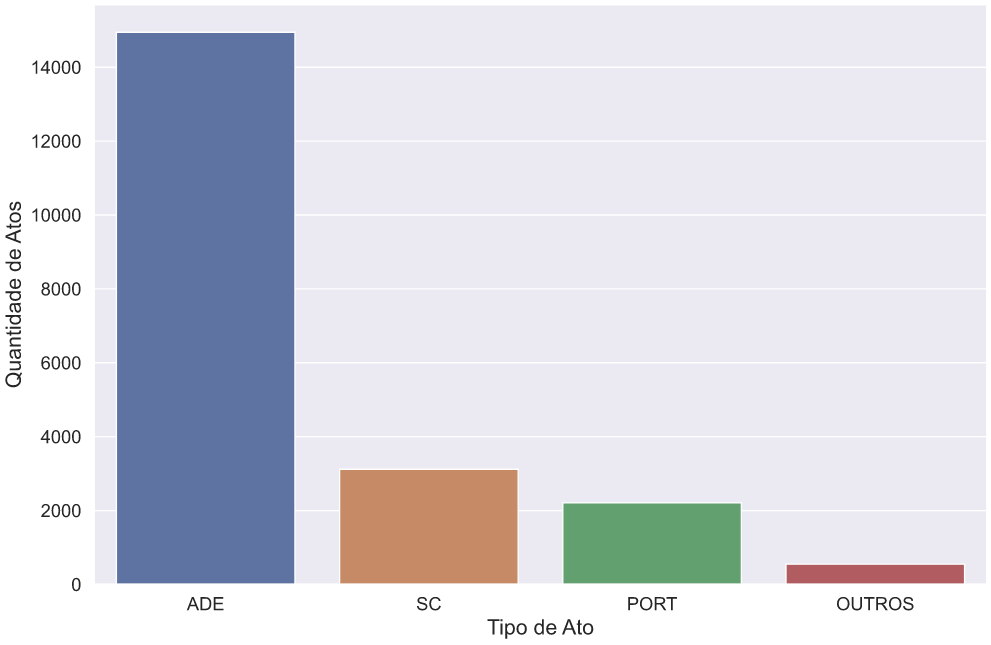
\includegraphics[scale=1.9]{exploratoria/atos-por-tipo-ato.png}
	\fdp
\end{figure}

Outro ponto importante analisado foi a distribuição dos segmentos por tipo de ato e tipo de segmento. Na tabela \ref{tab:segmentos-por-tipo} é possível perceber que dos 17 tipos possíveis de segmento, somente 13 estão presentes em atos dos tipos ADE, SC e PORT. Além disso, nem todos os 13 tipos de segmento estão presentes nos 3 tipos de ato e alguns tipos de segmento são pouco frequentes.

\begin{table}[h] 
\caption{Quantidade de segmentos por tipo de ato e tipo de segmento}
\label{tab:segmentos-por-tipo}
	\begin{center} 

		\begin{tabular}{rrrr}
		\toprule
		TIPO DE ATO &      ADE    &   PORT &      SC \\
		TIPO DE SEGMENTO          &        &         \\
		\midrule
		Alínea           &    780 &  2.265 &      87 \\
		Artigo           & 37.921 & 11.578 &       3 \\
		Autor            &      3 &      4 &       0 \\
		Capítulo         &      5 &    381 &       0 \\
		Ementa           & 14.948 &  2.207 &   3.119 \\
		Fecho            & 14.853 &  2.289 &     919 \\
		Inciso           &  4.134 & 17.399 &       0 \\
		Item             &    398 &    388 &      10 \\
		Não Identificado & 36.288 & 11.726 &   6.609 \\
		Parágrafo        &    861 &  5.894 &       0 \\
		Seção            &      3 &    219 &       0 \\
		SubSeção         &      0 &     18 &       0 \\
		Título           &    545 &    540 &       0 \\
		\bottomrule
	\end{tabular}
	\end{center}
	\fdp
\end{table} 

Os segmentos do tipo ``Não Identificado'' representam um ponto de atenção para a classificação dos segmentos. Por ser o tipo padrão de segmento do sistema Normas, sempre que ocorre falha humana por omissão na classificação manual, o segmento fica classificado como ``Não Identificado''. Apesar disso, essa é uma classe válida de segmento amplamente utilizada para representar trechos do ato que não precisam de formatação específica. Por pertencerem a um dos tipos mais frequentes de segmento, os segmentos ``Não Identificados'' não podem ser removidos do escopo da classificação, mas a presença de segmentos com classificação omissa pode prejudicar os resultados dos modelos.

\subsection{Identificação de Padrões\label{sec:identificacao-padroes-regex}}

Ao longo da análise exploratória foram identificados, em alguns tipos de segmento, padrões de texto  que podem ser utilizados como heurísticas baseadas em expressões regulares. Se essas heurísticas apresentarem resultados melhores do que o modelo de classificação, será possível retirar alguns tipos de segmento do escopo da classificação, deixando o modelo mais específico para as demais classes. A seguir são apresentados os padrões encontrados:

\begin{alineas}
	\item Artigos iniciam com a abreviação ``Art.'' seguida de um numeral ordinal. Exemplo: ``Art. 2\textsuperscript{o} O detalhamento do motivo da exclusão poderá ser obtido[...]'';
	\item Incisos são iniciados com um numeral romano seguido de hífem. Exemplo: ``IV – Fundamento legal para reconhecimento do direito[...]'';
	\item Alíneas iniciam com letras (minúsculas ou maiúsculas) seguidas de parênteses. Exemplo: ``f) desempenhar as tarefas inerentes ao sistema de progressão funcional[...]'';
	\item Parágrafos podem ser iniciados com a expressão ``Parágrafo único'' ou com o símbolo ``§'' seguido de um numeral ordinal. Exemplo: ``§ 2\textsuperscript{o} Compete à chefia imediata a gestão da frequência dos seus servidores[...]''.
\end{alineas}

 \subsection{Conclusões da Análise Exploratória}
 
 Ao final da análise exploratória de dados foi possível elencar as seguintes conclusões que serviram de base para as etapas seguintes do fluxo de aprendizado de máquina:

\begin{alineas}
	\item Os segmentos do tipo Anexo podem ser removidos do conjunto de dados por não representarem conteúdo textual;
	\item Os segmentos com valores ausentes são pouco representativos (0,06\% do total de segmentos) e podem ser removidos do conjunto de dados;
	\item Será necessário tratar caracteres inválidos na etapa de limpeza;
	\item Os tipos de ato ADE, SC e PORT representam 97,37\% do total de atos. Os demais tipos de ato juntos são bem menos frequentes e podem ser removidos do conjunto de dados;	 
	\item Os tipos de segmento (variável alvo da classificação) variam de um tipo de ato para outro e isso precisa ser considerado nas etapas seguintes;
	\item Existem padrões nos textos de alguns tipos de segmento que permitem a avaliação de heurísticas alternativas à utilização de algoritmos de classificação.
\end{alineas}

\section{Limpeza de Dados}

A etapa de limpeza de dados é responsável por excluir dados com valores inválidos ou pouco representativos. Os principais pontos identificados na análise exploratória de dados foram a exclusão de atos que não pertençam aos tipo ADE, SC e PORT, a remoção de segmentos do tipo Anexo, a eliminação de valores ausentes e a exclusão de caracteres de \textit{escape} e \textit{tags} HTML.

A classe LimpezaDados (limpeza\textunderscore dados.py) é responsável por buscar os dados provenientes da etapa de coleta (já carregados no objeto de dados), realizar as tarefas de limpeza e gravar os dados de volta no objeto de dados. Os atributos \textbf{orig} e \textbf{limp} definidos na classe Dados armazenam  respectivamente os dados da coleta e os dados após a limpeza. O código a seguir apresenta um exemplo de execução da etapa de limpeza a partir do notebook fluxo-ml.ipynb:

\begin{lstlisting}
	lp = LimpezaDados(dados)
	lp.executar(dados, 'ADE')
	12:57:52 - Excluindo segmentos dos atos que nao sao ADE...
	12:57:52 - 91448 segmentos de atos nao ADE excluidos.
	12:57:52 - Restaram 115040 segmentos de atos ADE.
	12:57:52 - Removendo segmentos nao representativos...
	12:57:52 - 6827 segmentos nao representativos excluidos.
	12:57:52 - Restaram 108213 segmentos representativos.
	12:57:52 - Removendo segmentos nulos...
	12:57:52 - 69 segmentos nulos excluidos.
	12:57:52 - Restaram 108144 segmentos nao nulos.
	12:57:52 - Removendo tags HTML...
	12:57:52 - Removendo caracteres de escape HTML...
	12:57:52 - Limpeza de dados concluida.
\end{lstlisting}

Na etapa de limpeza não é mais necessário instanciar o objeto de dados pois a etapa de carga já realizou essa tarefa. Dessa forma, o primeiro passo da limpeza é criar uma instância da classe LimpezaDados, chamando então o método ``executar'' e passando o objeto de dados como parâmetro. 

O tipo de ato precisa ser fornecido como parâmetro adicional. Isso ocorre porque, durante a análise exploratória de dados (seção \ref{sec:dist-atos-segmentos}), ficou evidente que alguns tipos de segmento não ocorreram para alguns tipos de ato ou ocorreram com uma frequência muito baixa. Como o tipo de segmento é a variável alvo para o modelo de classificação, remover os tipos de segmentos menos frequentes ou ausentes para um tipo de ato reduz a quantidade de classes do modelo, tornando-o mais específico para as classes mais frequentes. O tipo de ato é previamente conhecido (ou pode ser facilmente deduzido), logo, fornecer o tipo do ato como parâmetro não representa um desafio. 

Esses fatores acabaram direcionando a estratégia de classificação para a criação de modelos específicos de acordo com o tipo de ato. Dessa forma, os Atos Dclaratórios Executivos (ADE) tiveram um modelo de classificação específico, assim como as Soluções de Consulta (SC) e também as Portarias (PORT). Cado um desses modelos teve como domínio da variável alvo o conjunto de tipos de segmento pertencentes aquele tipo de ato. Nesse cenário, para os atos do tipo ADE, por exemplo, foram considerarados como variável alvo os tipos de segmento Artigo, Ementa, Fecho, Inciso e Não Identificado enquanto para os atos do tipo SC foram contemplados os segmentos do tipo Ementa, Fecho e Não Identificado. O limite de corte utilizado foi um valor menor do que 0,01 (1\%), calculado usando a fórmula a seguir:

\[ corte = \frac{qtd\_segmentos}{total\_segmentos} \]

\begin{quote}
Sendo \( corte \) o limite de corte dos segmentos, \( qtd\_segmentos \) a quantidade de segmentos encontrados (\textbf{de um determinado tipo de segmento}) para o tipo de ato informado e \( total\_segmentos \) a quantidade de segmentos encontrados (\textbf{de todos os tipos de segmento}) para o tipo de ato informado.
\end{quote}

Isso acabou trazendo uma tarefa adicional para a etapa de limpeza: remover os atos e segmentos não relacionados ao tipo de ato informado. Assim, a partir do parâmetro tipo\textunderscore ato, a classe de limpeza realiza duas tarefas: 
\begin{alineas}
	\item Exclui os atos (e seus segmentos) de tipos diferentes do indicado pelo parâmetro tipo\textunderscore ato (exemplo: se tipo\textunderscore ato='SC', excluir todos os atos 'ADE', 'PORT' e 'OUTROS';
	\item Remove os segmentos que pertencem a tipos de segmento não relacionados (por ausência ou baixa frequência) ao tipo de ato indicado pelo parâmetro tipo\textunderscore ato (exemplo: se tipo\textunderscore ato='SC', remover todos os segmentos que não sejam Ementa, Fecho ou Não Identificado).
\end{alineas}

No exemplo de código mencionado anteriormente, o parâmetro tipo\textunderscore ato foi igual a 'ADE', logo, foram removidos 91.448 segmentos de atos que não eram ADE e 6.827 segmentos dos tipos Autor, Capítulo, Item, Parágrafo, Seção, Subseção e Título, não representativos para os atos do tipo ADE, conforme informado na tabela \ref{sec:dist-atos-segmentos}. 
\section{Preprocessamento}

O preprocessamento é a etapa responsável por adequar a representação dos dados a um formato adequado aos algoritmos de aprendizado de máquina. Esta etapa contempla uma série de tarefas como remoção de pontuação, exclusão de \textit{stopwords}, tokenização,  \textit{steeming} e vetorização.

A classe Preprocessamento (preprocessamento.py) realiza as tarefas necessárias ao preprocessamento dos dados. Seguindo a mesma lógica das etapas anteriores, o objeto de dados (instância da classe Dados) traz os dados provenientes da etapa de Limpeza (atributo \textbf{limp}) e armazena os resultados do preprocessamento no atributo \textbf{prep}.  

\subsection{Remoção de Pontuação}

Caracteres de pontuação geralmente não contribuem com o resultado de algoritmos de classificação por serem muito repetitivos e guardarem pouca ou nenhuma informação específica de uma classe. Para a remoção dos caracteres de pontuação foi utilizada a coleção de carecteres \textit{punctuation}, parte da biblioteca padrão do Python e acessível através do módulo \textit{string}. Para remover os caracteres de pontuação foi necessário somente ler os textos dos segmentos e eliminar os caracteres do texto que pertenceciam à coleção \textit{punctuation}.

\subsection{Exclusão de \textit{Stopwords}}

\textit{Stopwords} são termos comuns em uma linguagem, como artigos e preposições, que não trazem contribuição para o resultado de algoritmos de classificação, de forma similar ao que ocorre com os caracteres de pontuação. Tanto no caso da pontuação, quanto no caso das \textit{stopwords}, a remoção dos termos permite uma redução do vocabulário, simplificando a representação do texto e permitindo uma atuação mais específica dos algoritmos de classificação. Para exclusão das \textit{stopwords} foi utilizada a coleção \textit{nltk.corpus.stopwords.words} em português do NLTK (\textit{Natural Language Toolkit})\footnote{https://www.nltk.org/}, uma biblioteca com diversas funções para o processamento de linguagem natural.

\subsection{Tokenização}

Tokenização é a tarefa de subdividir o texto em seus elementos fundamentais ou \textit{tokens}. A tokenização permite a identificação do conjunto de termos únicos que compõem o texto (o vocabulário), permitindo a aplicação de funções específicas termo-a-termo (como as funções de \textit{steeming}). Para realização da tokenização foi utilizada a biblioteca \textit{RegexpTokenizer} do NLTK que executa uma tokenização baseada em expressões regulares. Foram testados outras bibliotecas de tokenização do NLTK como o \textit{WhitespaceTokenizer} e o \textit{WordPunctTokenizer}, mas ambos apresentaram resultados inferiores de tokenização.

\subsection{Steeming}

\textit{Steeming} é a redução de um palavra ao seu radical, ou seja, a exclusão de sufixos presentes em variações de uma mesma palavra. As palavras menino, menina, meninos,  meninas, menininho, menininha e meninice, após um processo de \textit{steeming}, seriam reduzidas ao radical \textbf{menin}. Esta eliminação das variações permite tratar diferentes palavras como um único \textit{token}, reduzindo o vocabulário e consequentemente o espaço de estados das caraterísticas de entrada dos modelos de classificação. Para realização do processo de \textit{steeming} foi utilizado o \textit{SnowballStemmer} do NLTK.

\subsection{Vetorização}

A vetorização ou extração de características converte o texto para uma representação matemática que possa ser utilizada como entrada para os algoritmos de aprendizado de máquina. 
\endgroup

\newpage

% ----------------------------------------------------------
% ELEMENTOS PÓS-TEXTUAIS
% ----------------------------------------------------------
\postextual

% Referências bibliográficas
\bibliography{referencias}

\end{document}
